% slides.tex
\documentclass[20pt]{beamer}
\usepackage{listings}
\usepackage[utf8]{inputenc}
\usepackage{color}
\usepackage{graphicx}

\usetheme{default}
\usecolortheme{dove}
\useoutertheme{default}

% Slightly smaller title
\setbeamerfont{frametitle}{size=\large}
\setbeamerfont{verb}{size=\small}

% lst settings
\lstset{
    language=Haskell,
    basicstyle=\small,
    gobble=4
}

\newcommand{\vspaced}{
    \vspace{5mm}
}

\begin{document}

\title{Porting Text to UTF-8}
\subtitle{Dutch Haskell User Group}
\author{Jasper Van der Jeugt}
\date{July 14, 2011}

\begin{frame}[plain]
    \titlepage
\end{frame}

% Introduction
% ------------

\begin{frame}{Hello!}
    My name is Jasper \\
    Student at UGent \\
    I write Haskell \\
    GhentFPG \\
    \texttt{@jaspervdj} \\
    \texttt{jaspervdj.be}
    \begin{picture}(0.0, 0.0)
    \put(40.0, -15.0){
        
\includegraphics[width=0.5\textwidth]{../2011-functionalpx-blaze-html/images/hat.pdf}}
    \end{picture}
\end{frame}

\begin{frame}{Overview}
    Credit where credit is due \\
    \vspaced
    \textit{High-Performance Haskell}, advice \\
    Johan Tibell \\
    \vspaced
    Mentoring \\
    Edward Kmett
\end{frame}

\begin{frame}{Overview}
    \textbf{Introduction} \\
    UTF-8 vs. UTF-16 \\
    Porting Text to UTF-8 \\
    Benchmarking pitfalls \\
    GHC Core \\
    Results
\end{frame}

% UTF-8 vs. UTF-16
% ----------------

\begin{frame}{Overview}
    Introduction \\
    \textbf{UTF-8 vs. UTF-16} \\
    Porting Text to UTF-8 \\
    Benchmarking pitfalls \\
    GHC Core \\
    Results
\end{frame}

\begin{frame}{UTF-8 vs. UTF-16}
    \textbf{Number of unicode characters?} \\
    \vspaced
    17 planes \\
    Each plane: $2^{16}$ characters \\
\end{frame}

\begin{frame}{UTF-8 vs. UTF-16}
    \textbf{Number of unicode characters?} \\
    \vspaced
    $17 * 2^{16}$ characters \\
\end{frame}

\begin{frame}{UTF-8 vs. UTF-16}
    \textbf{Number of bits needed?} \\
    \vspaced
    $\log_2(17 * 2^{16}) = 20.087...$ \\
    \vspaced
    21 bits per character \\
\end{frame}

\begin{frame}[fragile]{UTF-8 vs. UTF-16}
    \textbf{String is (often) a bad choice} \\
    \vspaced
    \begin{lstlisting}
    data Char = C# Char#
    \end{lstlisting}
    \texttt{C\#}: word \\
    \texttt{Char\#}: 32 bits \\
\end{frame}

\begin{frame}[fragile]{UTF-8 vs. UTF-16}
    \textbf{String is (often) a bad choice} \\
    \vspaced
    \begin{lstlisting}
    data [] a = [] | a : [a]
    \end{lstlisting}
\end{frame}

\begin{frame}{UTF-8 vs. UTF-16}
    \begin{center}
    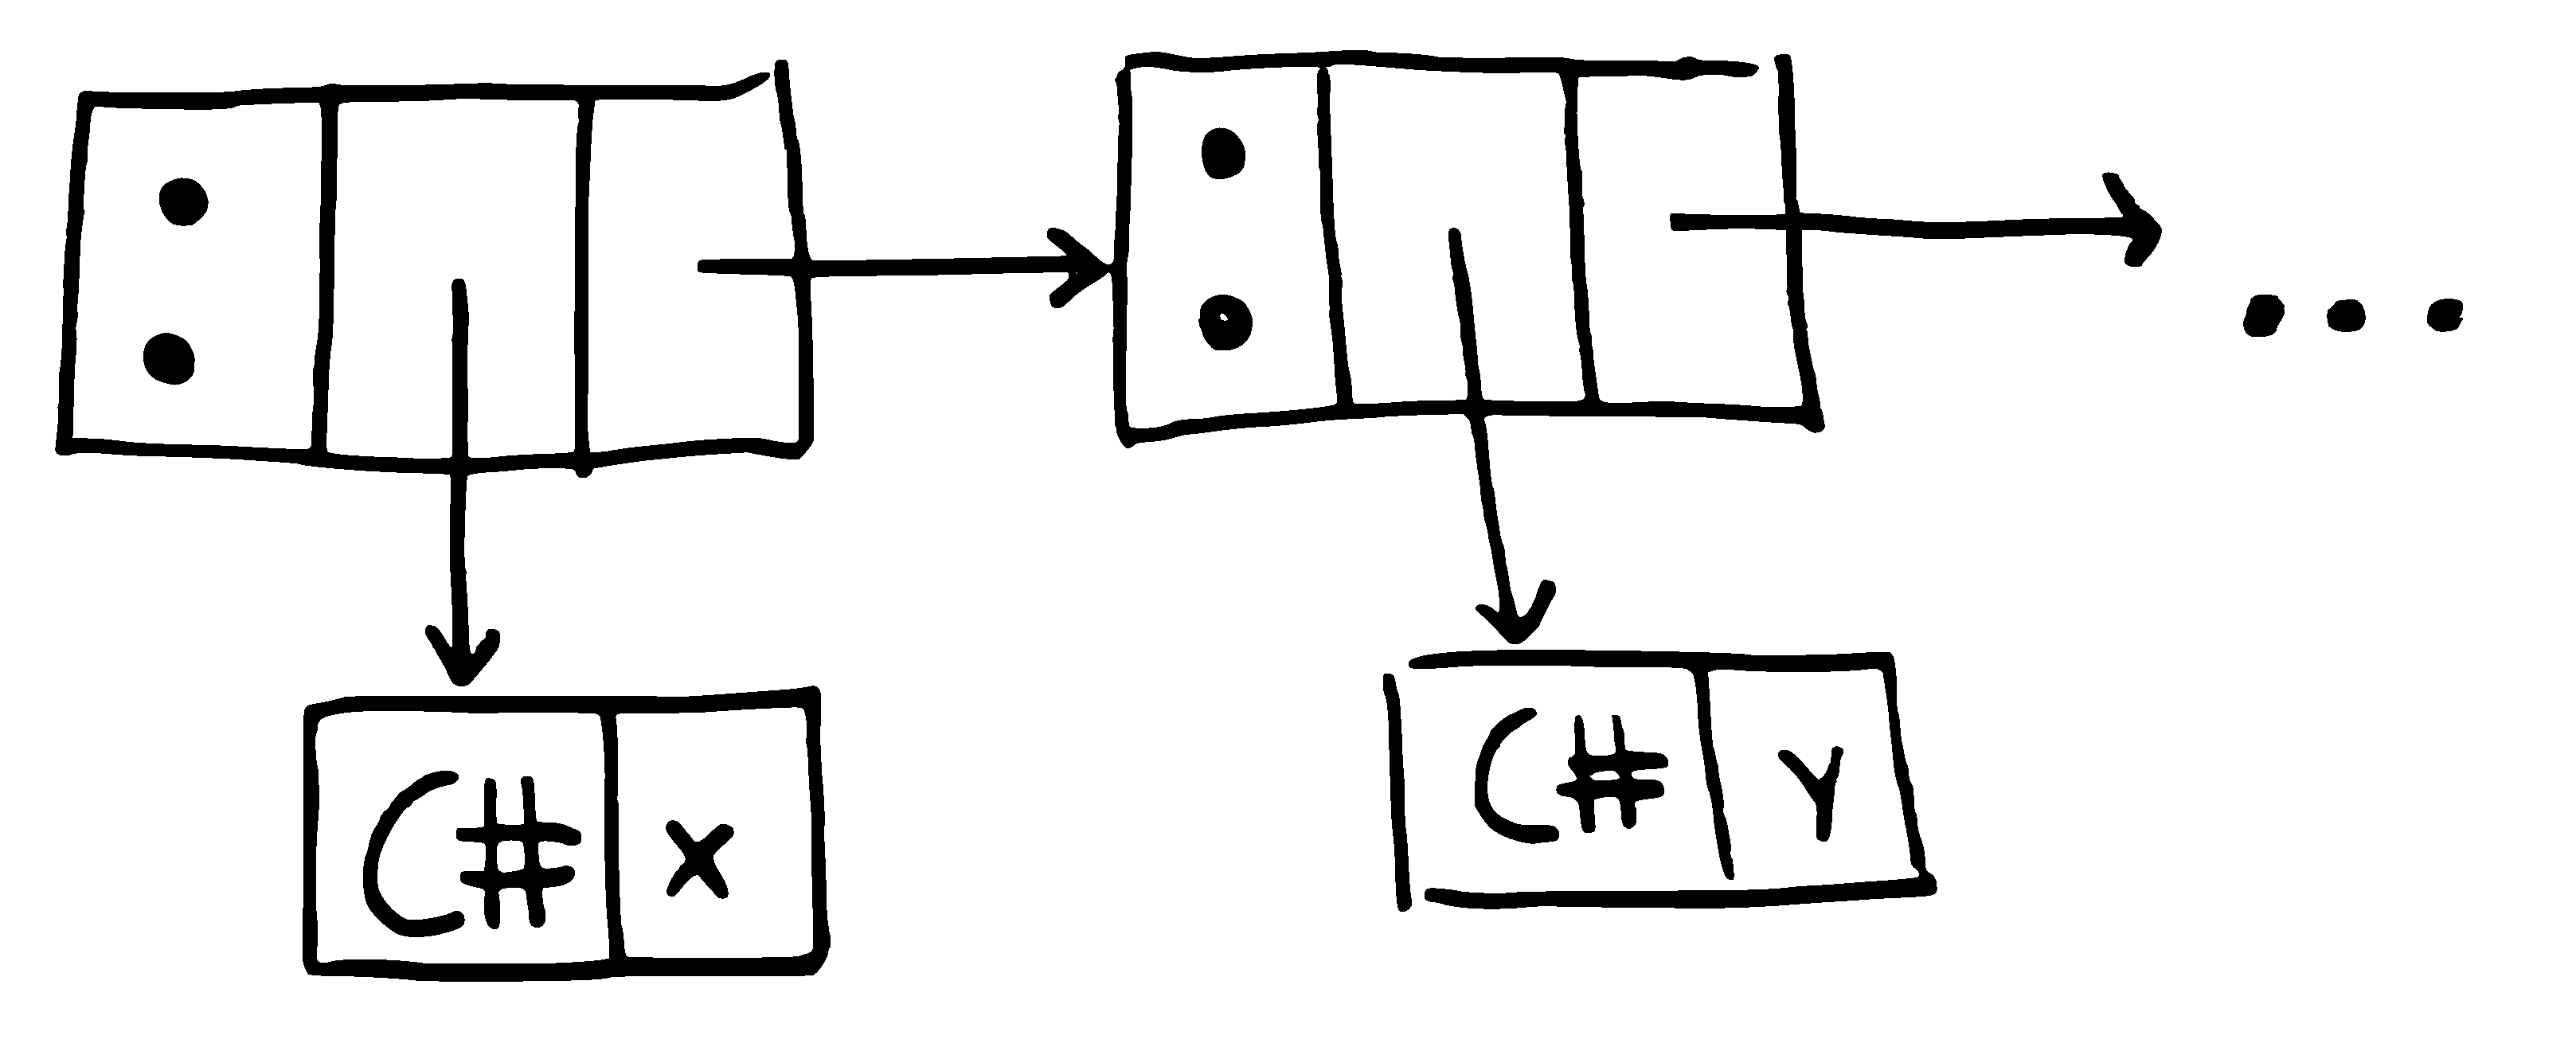
\includegraphics[width=\textwidth]{images/string.pdf}
    \end{center}
\end{frame}

\begin{frame}{UTF-8 vs. UTF-16}
    Two points: \\
    \begin{enumerate}
    \item Use strict arrays
    \item Don't use a 32-bit encoding
    \end{enumerate}
\end{frame}

\begin{frame}{UTF-8 vs. UTF-16}
    \begin{center}
    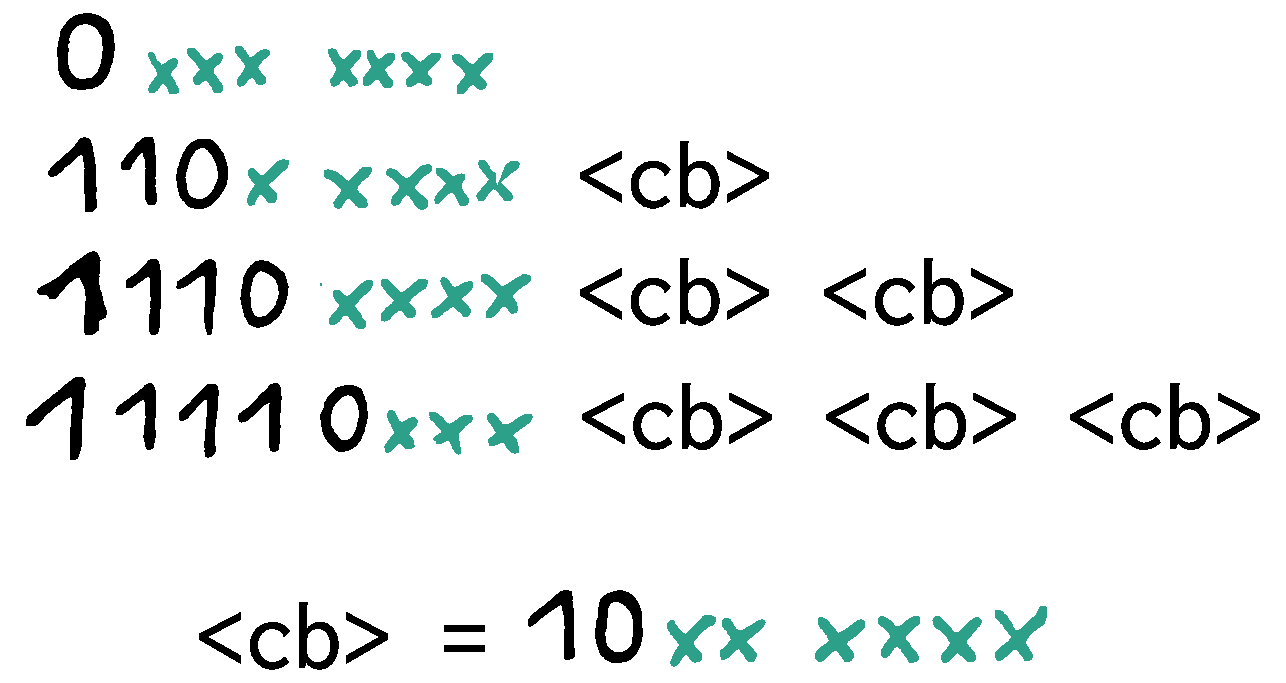
\includegraphics[width=0.9\textwidth]{images/utf8.pdf}
    \end{center}
\end{frame}

\begin{frame}{UTF-8 vs. UTF-16}
    \begin{center}
    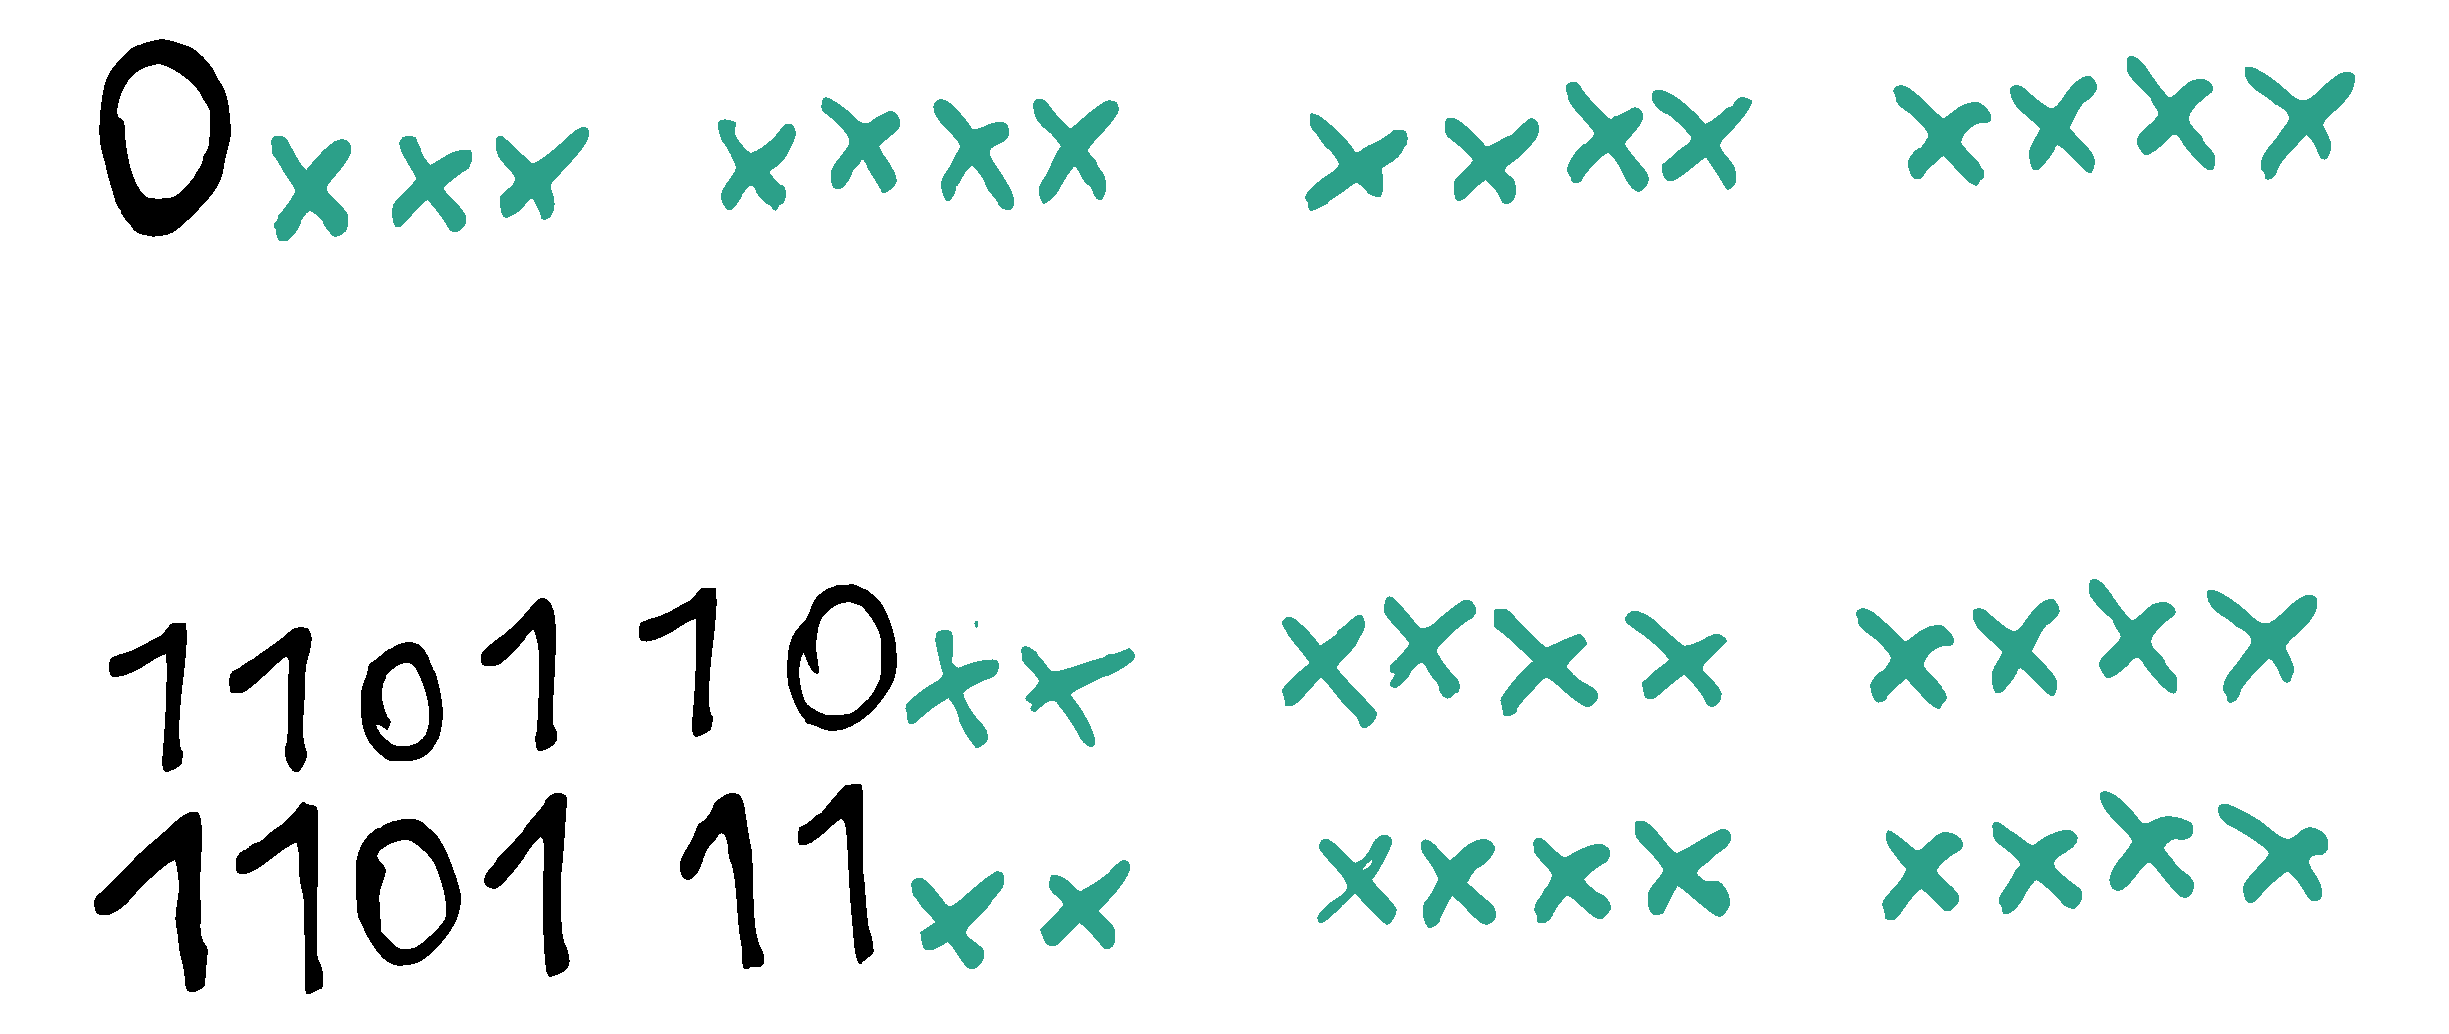
\includegraphics[width=0.9\textwidth]{images/utf16.pdf}
    \end{center}
\end{frame}

\begin{frame}{UTF-8 vs. UTF-16}
    Two points:
    \begin{enumerate}
    \item Some things are inherently faster using UTF-8
    \item Some things are inherently faster using UTF-16
    \end{enumerate}
\end{frame}

% Porting Text to UTF-8
% ---------------------

\begin{frame}{Overview}
    Introduction \\
    UTF-8 vs. UTF-16 \\
    \textbf{Porting Text to UTF-8} \\
    Benchmarking pitfalls \\
    GHC Core \\
    Results
\end{frame}

\begin{frame}[fragile]{Porting Text to UTF-8}
    \begin{lstlisting}
    encodeUtf8 :: Text -> ByteString
    \end{lstlisting}
    \vspaced
    Implementation very simple
\end{frame}

\begin{frame}[fragile]{Porting Text to UTF-8}
    \begin{lstlisting}
    encodeUtf8 (Text arr off len) =
      unsafePerformIO $ do
        fp <- mallocByteString len
        withForeignPtr fp $ <memcpy>
        return $! PS fp 0 len
    \end{lstlisting}
\end{frame}

\begin{frame}[fragile]{Porting Text to UTF-8}
    \begin{lstlisting}
    decodeUtf8 :: ByteString -> Text
    \end{lstlisting}
    \vspaced
    Very important to validate first!
\end{frame}

\begin{frame}{Porting Text to UTF-8}
    \texttt{decodeUtf8 =}
    \vspaced
    \begin{center}
    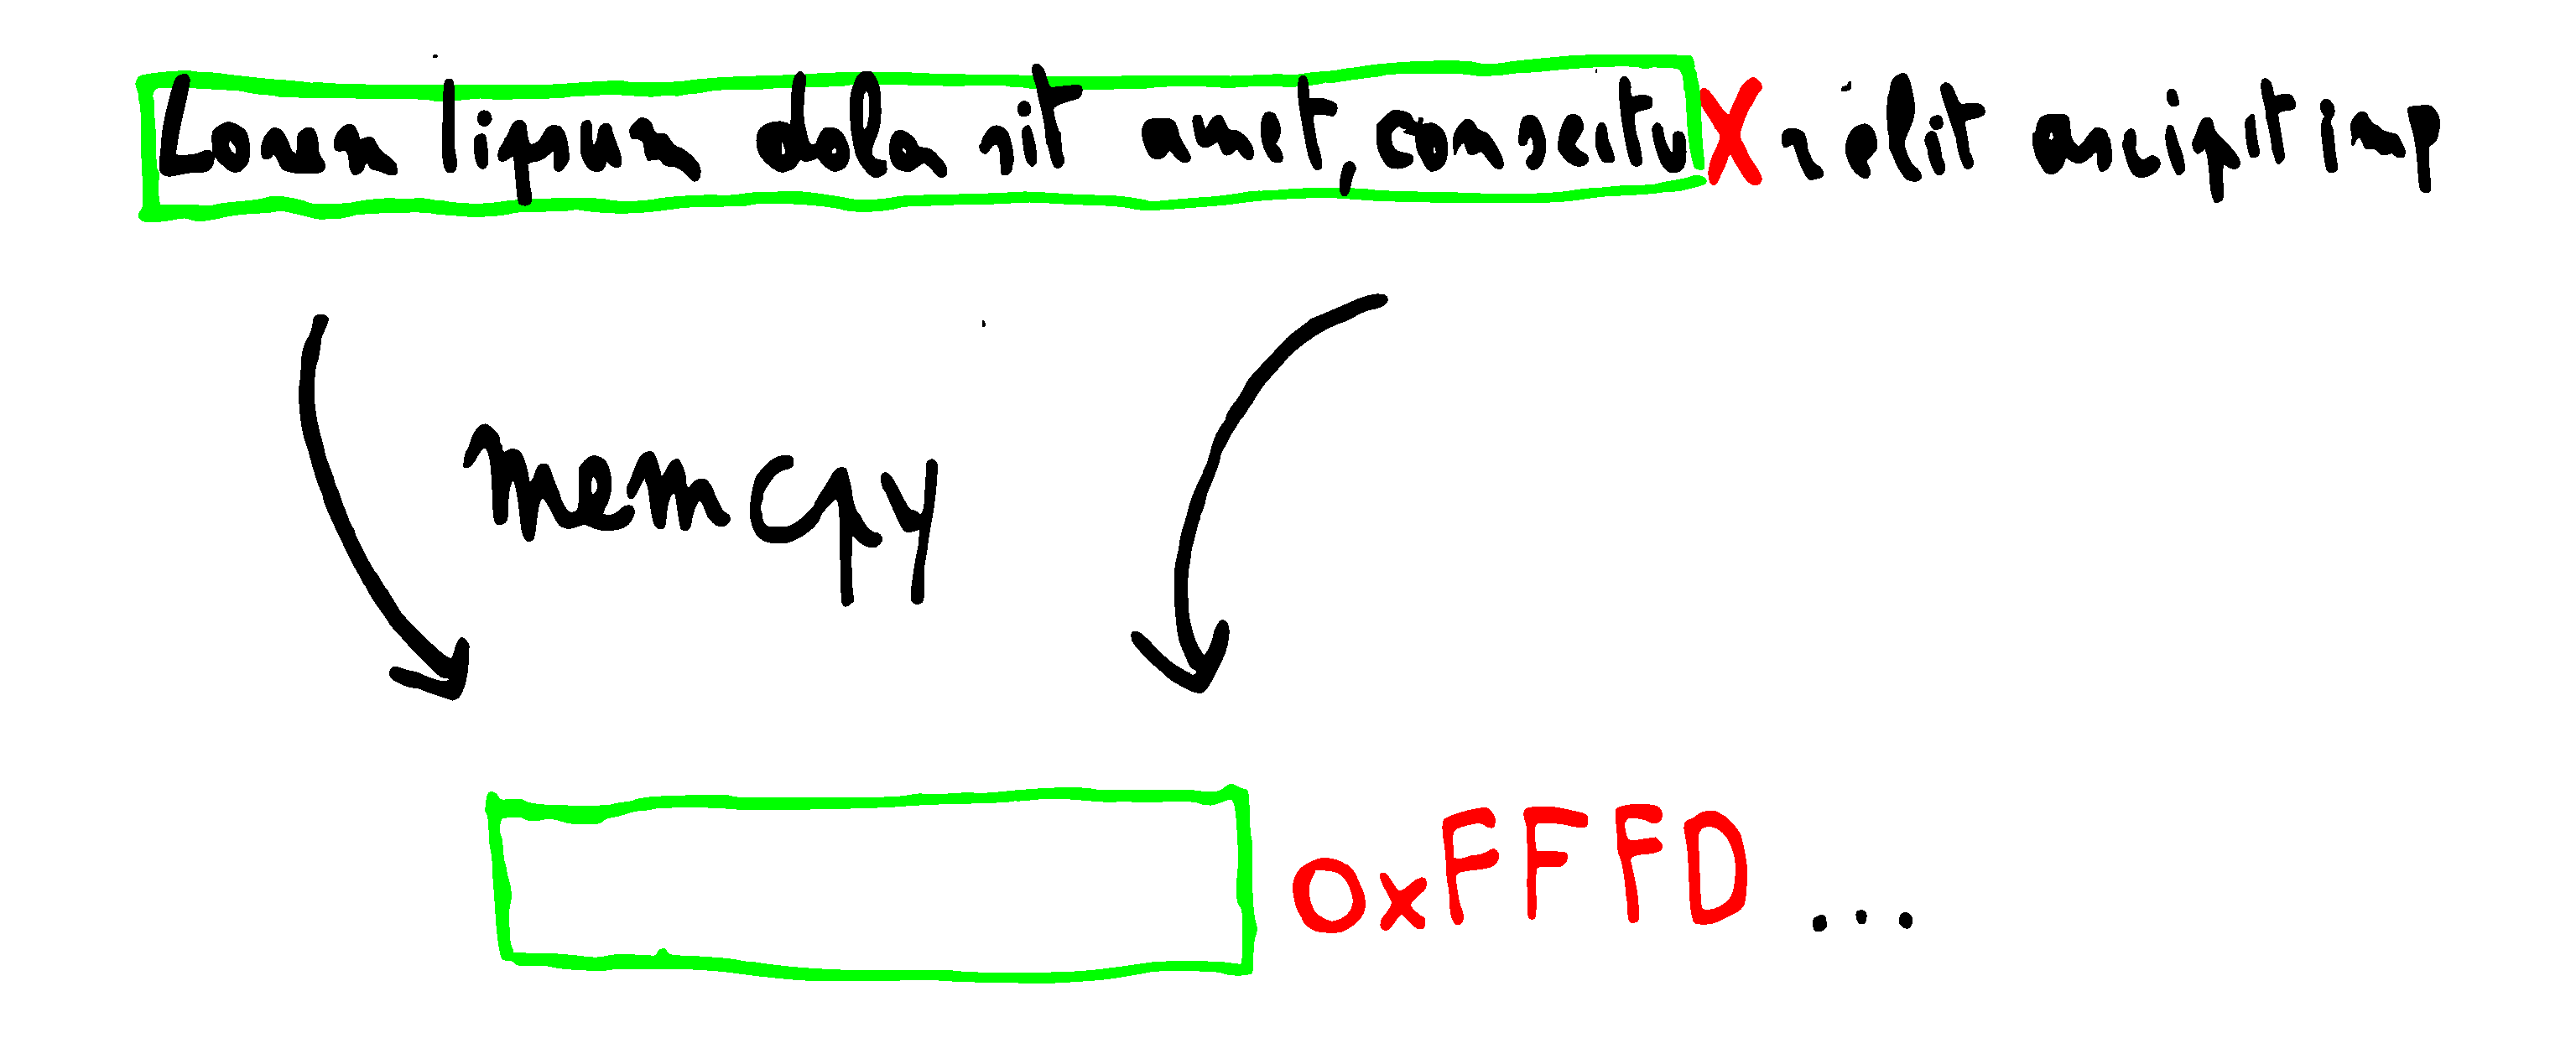
\includegraphics[width=\textwidth]{images/decode.pdf}
    \end{center}
\end{frame}

\begin{frame}[fragile]{Porting Text to UTF-8}
    Implementations of \texttt{map}, \texttt{filter}...
    \vspaced
    \begin{lstlisting}
    stream   :: Text -> Stream Char
    unstream :: Stream Char -> Text
    \end{lstlisting}
\end{frame}

\begin{frame}[fragile]{Porting Text to UTF-8}
    \begin{lstlisting}
    data Stream a =
        forall s. Stream
        (s -> Step s a) -- stepper
        !s              -- state
        !Size           -- size hint
    \end{lstlisting}
\end{frame}

\begin{frame}[fragile]{Porting Text to UTF-8}
    \begin{lstlisting}
    data Step s a
        = Done
        | Skip !s
        | Yield !a !s
    \end{lstlisting}
\end{frame}

\begin{frame}[fragile]{Porting Text to UTF-8}
    Most functions written as:
    \vspaced
    \begin{lstlisting}
    f :: Text -> Text
    f = unstream . f' . stream
    \end{lstlisting}
\end{frame}

\begin{frame}[fragile]{Porting Text to UTF-8}
    \begin{lstlisting}
    f = unstream . f' . stream
    g = unstream . g' . stream
    \end{lstlisting}
    \vspaced
    Stream fusion: \\
    \begin{lstlisting}
    f . g =
        unstream . f' . g' . stream
    \end{lstlisting}
\end{frame}

\begin{frame}[fragile]{Porting Text to UTF-8}
    These are not the only streaming combinators...
    \vspaced
    \begin{lstlisting}
    stream . decodeUtf8 = streamUtf8
    \end{lstlisting}
    \vspaced
    \begin{lstlisting}
    streamUtf8 ::
        ByteString -> Stream Char
    \end{lstlisting}
\end{frame}

% Benchmarking pitfalls
% ---------------------

\begin{frame}{Overview}
    Introduction \\
    UTF-8 vs. UTF-16 \\
    Porting Text to UTF-8 \\
    \textbf{Benchmarking pitfalls} \\
    GHC Core \\
    Results
\end{frame}

\begin{frame}{Benchmarking pitfalls}
    Haskell is a lazy language \\
    This makes benchmarking hard
\end{frame}

\begin{frame}{Benchmarking pitfalls}
    Two types of benchmarks: \\
    Functions and programs \\
    \vspaced
    (we focus on the former)
\end{frame}

\begin{frame}[fragile]{Benchmarking pitfalls}
    Benchmarking some function

    \begin{lstlisting}
    f :: Int -> Int
    \end{lstlisting}
\end{frame}

\begin{frame}[fragile]{Benchmarking pitfalls}
    In e.g. Python
    \vspaced
    \begin{lstlisting}
    total = 0
    for i in range(100):
        start = time.time()
        f()
        end = time.time()
        total += (end - start) / 100
    \end{lstlisting}
\end{frame}

\begin{frame}[fragile]{Benchmarking pitfalls}
    In Haskell?
    \vspaced
    \begin{lstlisting}
    replicateM 100 $ do
        start <- getTime
        let y = f x
        end <- y `seq` getTime
    \end{lstlisting}
    \vspaced
    This is pretty hard to get right
\end{frame}

\begin{frame}{Benchmarking pitfalls}
    Conclusion? \\
    \vspaced
    \textbf{Never write your own benchmarking code}
\end{frame}

\begin{frame}{Benchmarking pitfalls}
    \textbf{Criterion} \\
    \vspaced
    By Bryan O'Sullivan
\end{frame}

\begin{frame}[fragile]{Benchmarking pitfalls}
    Criterion \\
    \vspaced
    \begin{lstlisting}
    bench "f" $ nf   f x
    bench "g" $ whnf g x
    \end{lstlisting}
\end{frame}

\begin{frame}[fragile]{Benchmarking pitfalls}
    \texttt{Eq} for string types \\
    \vspaced
    \begin{lstlisting}
    whnf (== T.init t
        `T.snoc` '\xfffd') t

    whnf (== BL.init bl
        `BL.snoc` '\xfffd') bl
    \end{lstlisting}
\end{frame}

\begin{frame}{Benchmarking pitfalls}
    But \texttt{ByteString.Lazy} \\
    is a little faster \\
    \vspaced
    \texttt{Text}: 2.489305 us
    \texttt{ByteString.Lazy}: 39.29312 \textbf{ns}
\end{frame}

\begin{frame}[fragile]{Benchmarking pitfalls}
    Digging into the code... \\
    \vspaced
    \begin{lstlisting}
    eq (Chunk a as) (Chunk b bs) =
      case compare (S.length a)
                   (S.length b) of
        ...
        EQ -> a == b && eq as bs
        ...
    \end{lstlisting}
\end{frame}

\begin{frame}[fragile]{Benchmarking pitfalls}
    Digging further... \\
    \vspaced
    \begin{lstlisting}
    eq a@(PS p s l) b@(PS p' s' l')
       -- short cut on length
       | l /= l'            = False
       -- short cut for same string
       | p == p' && s == s' = True
       | ...
    \end{lstlisting}
\end{frame}

\begin{frame}{Benchmarking pitfalls}
    Conclusion? \\
    \vspaced
    \textbf{Libraries can be smarter than you think they are, make sure you know
    what you are benchmarking!}
\end{frame}

\begin{frame}[fragile]{Benchmarking pitfalls}
    Benchmarking IO \\
    \vspaced
    \begin{lstlisting}
    bench "HtmlCombinator" $ do
      putStr "Content-Type: ..."
      ...
      putStr "<table>"
      putStr $ toLazyText $
        makeTable 20000
      putStr "</table>"
    \end{lstlisting}
\end{frame}

\begin{frame}[fragile]{Benchmarking pitfalls}
    This looks suspicious \\
    \vspaced
    \begin{lstlisting}
    benchmarking HtmlCombinator
    collecting 100 samples (...)
        estimated 30.80161 s
    mean: 107.6378 ms (...)
    \end{lstlisting}
    \vspaced
    $100 * 100ms \neq 30s$
\end{frame}

\begin{frame}{Benchmarking pitfalls}
    \begin{center}
    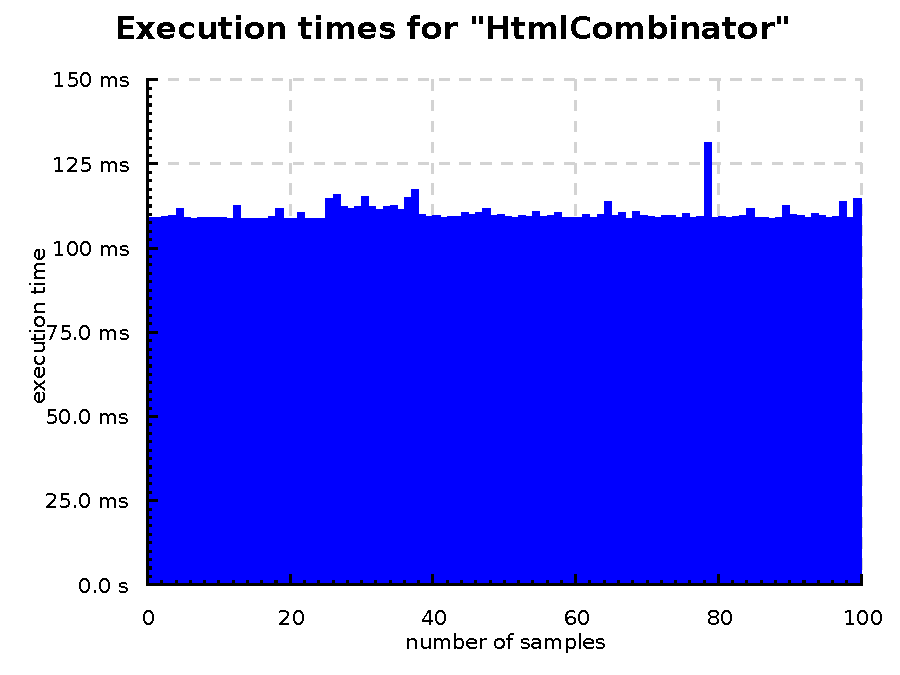
\includegraphics[width=0.9\textwidth]{images/htmlcombinator.pdf}
    \end{center}
\end{frame}

\begin{frame}[fragile]{Benchmarking pitfalls}
    Where is the issue? \\
    \vspaced
    \begin{lstlisting}
    bench "HtmlCombinator" $ do
      putStr "Content-Type: ..."
      ...
      putStr "<table>"
      putStr $ toLazyText $
        makeTable 20000
      putStr "</table>"
    \end{lstlisting}
\end{frame}

\begin{frame}[fragile]{Benchmarking pitfalls}
    \begin{lstlisting}
    putStr . toLazyText .
        makeTable =<< rows
    ...
    where
      rows :: IO Int
      rows = return 20000
      {-# NOINLINE rows #-}
    \end{lstlisting}
\end{frame}

\begin{frame}{Benchmarking pitfalls}
    Conclusion? \\
    \vspaced
    \textbf{GHC is pretty smart as well}
\end{frame}

% GHC Core
% --------

\begin{frame}{Overview}
    Introduction \\
    UTF-8 vs. UTF-16 \\
    Porting Text to UTF-8 \\
    Benchmarking pitfalls \\
    \textbf{GHC Core} \\
    Results
\end{frame}

\begin{frame}{GHC Core}
    What is GHC Core? \\
    Why should we care?
\end{frame}

\begin{frame}{GHC Core}
    \textbf{What is GHC Core?} \\
    \vspaced
    Internal representation used by GHC \\
    A kernel language \\
    Optimizations are applied here
\end{frame}

\begin{frame}{GHC Core}
    \textbf{Why should we care?} \\
    \vspaced
    Understanding benchmark results \\
    Know what is going on \\
    Impress your friends!
\end{frame}

\begin{frame}{GHC Core}
    A few basic rules
\end{frame}

\begin{frame}{GHC Core}
    Function pattern matching, guards, if's are translated to \texttt{case}
\end{frame}

\begin{frame}{GHC Core}
    \texttt{where} is translated to \texttt{let}
\end{frame}

\begin{frame}{GHC Core}
    Type annotations everywhere
\end{frame}

\begin{frame}{GHC Core}
    \textbf{Reading core} \\
    \vspaced
    Clean up qualified names \\
    Use proper variable names \\
    Remove unnecessary type annotations
\end{frame}

\begin{frame}{GHC Core}
    \textbf{Demo}
\end{frame}

% Results
% -------

\begin{frame}{Overview}
    Introduction \\
    UTF-8 vs. UTF-16 \\
    Porting Text to UTF-8 \\
    Benchmarking pitfalls \\
    GHC Core \\
    \textbf{Results}
\end{frame}

\begin{frame}[fragile]{Results}
    \begin{lstlisting}
    text <- T.decodeUtf8 <$>
      B.readFile filePath

    B.putStr $ T.encodeUtf8 $
      T.toUpper text
    \end{lstlisting}
\end{frame}

\begin{frame}{Results}
    \begin{center}
    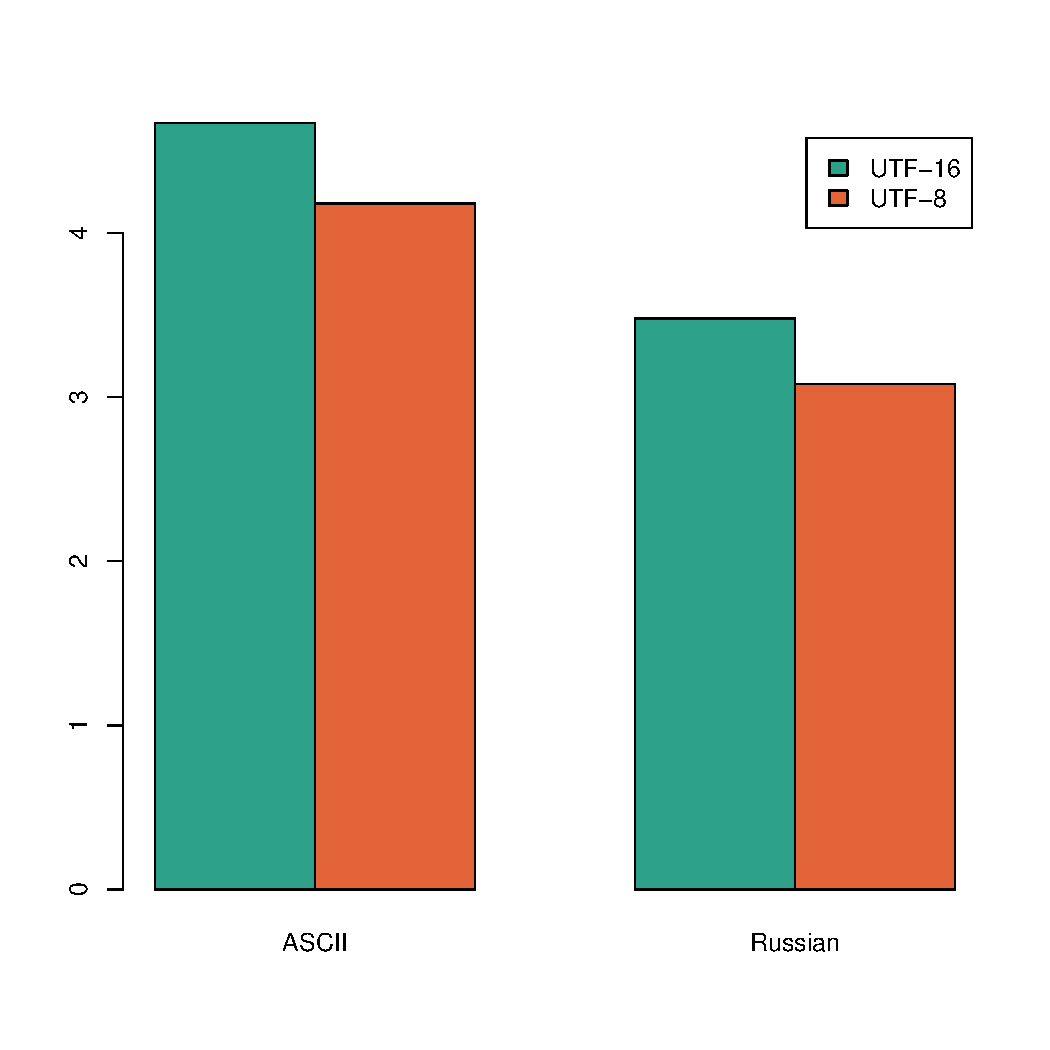
\includegraphics[width=0.75\textwidth]{images/upper.pdf}
    \end{center}
\end{frame}

\begin{frame}[plain]
    \begin{center}
    \huge{Questions?}
    \end{center}
\end{frame}

\end{document}
